\section{Einleitung und Zielsetzung}
\label{sec:Ziel}

\begin{wrapfigure}{r}{0.3\textwidth}
	\centering
	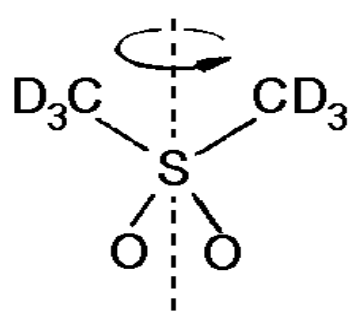
\includegraphics[width=0.25\textwidth]{Plots/Probe.png}
	\caption{Dimethylsulton-Kristall.}
	\label{probe}
\end{wrapfigure}
In diesem Versuch soll die Molek\"{u}l- und Ionendynamik von Dimethylsulton-Kristalle mittels magnetischer Kernresonanz (NMR) Spektroskopie untersucht werden.
Dazu wird ein Deuteronen-NMR verwendet.
Mit der magnetische Kernresonanz k\"{o}nnen unteranderem Informationen \"{u}ber dynamische Bewegungsprozesse ermittelt werden.
Ziel dieses Versuches ist es, die Relaxationszeiten $T_1$ und $T_2$ der vorliegenden Probe zu bestimmen.
Sowie stimulierte Echos fu\"{u}r verschiedene Temperaturen aufzunehmen.

%- Temperaturabh\"{a}ngigkeit
%- NMR - magnetische Kernresonanz -> Verfahren zur Strukturaufkl\"{a}rung
%- NMR ortsaufl\"{o}sendes Hilfsmittel in Medizin und Materialwissenschaften
%- neben Strukturinformation auch dynamische Informationen -> zeitlicher Verlauf von Bewegungsprozessen
%- rotatorische und translatorische Bewegungen von Molek\"{u}l(-gruppen)
%
%In diesem Versuch: Dimethylsulton-Kristalle, diese k\"{o}nnen $180^{\circ}$ Spr\"{u}nge ausf\"{u}hren
%- sonde: Deuteronen-NMR
